\documentclass[12pt]{article}
\usepackage{inputenc}
\usepackage[top=1in, bottom=1in, left=1in, right=1in]{geometry}
\usepackage{setspace}
\usepackage{parskip}
\setcounter{secnumdepth}{1}
\pagestyle{plain}
\usepackage{graphicx}
\setlength{\parindent}{0 cm}
\usepackage[compact]{titlesec}  
\usepackage{amssymb}
\usepackage{amsmath}
\usepackage{float}

\newcommand\numberthis{\addtocounter{equation}{1}\tag{\theequation}}
\titlespacing{\section}{0pt}{0pt}{0pt}


\begin{document}
\section*{Blood Cell Fixed Point Calculations}
Consider the blood cell iterative equation $c_{n+1} = (1-a)c_{n}+bc_{n}^{r}e^{-sc_{n}}$.

\textbf{Question 2:} Assuming that $b=1.1*10^{6}$, $r=8$ and $s=16$ show that there are two stable and one unstable fixed points of period one when $a=0.2$.

\textbf{Answer:} This question involves both a) finding the fixed points and b) determining the stability of these fixed points. 

Finding Fixed Points: Because we are solving for \emph{period one}, we can solve (a) by finding the intersection points of the line $y=x$ with $f(x) = (1-a)x+(1.1*10^{6})x^{8}e^{-16x}$. Usually we can determine these intersection points using numerical algorithms such as Newton's Method or the Secant Method. In this case, however, we found that these numerical methods failed to converge to the fixed points that were found graphically.

Using the following Matlab script, the functions and their derivatives were defined symbolically with the `symfun' function and plotted against $y=x$:

\begin{quote}
	\begin{verbatim}
% Set Parameters
a = .2; b = 1.1*10^6; r = 8; s = 16;
% Define Functions and Derivatives
syms x
f = symfun((1-a)*x+b*x^(r)*exp(-s*x),[x]); derivf = diff(f);
a = .3; g = symfun((1-a)*x+b*x^(r)*exp(-s*x),[x]); derivg = diff(g);
y = symfun(x,[x]);
% Plot F(x) vs Y(x)
h1 = ezplot(f,[-.01,1]); hold on; h2 = ezplot(y,[-.01,1]); 
set(h1,`color',`r',`linestyle',`--');
% Set Legend 
legend(`f(x)',`y = x'); xlabel(`x'); ylabel(`f(x) and y(x)');
title(`f(x) = (1-a)*x+b*x^(r)*exp(-s*x) against y(x) = x')
hold off
% Plot G(x) vs Y(x)
h3 = ezplot(g,[-.01,1]); hold on; h4 = ezplot(y,[-.01,1]);
set(h3,`color',`r',`linestyle',`--')
% Set Legend
legend(`g(x)',`y = x');; xlabel(`x'); ylabel(`g(x) and y(x)'); 
title(`g(x) = (1-a)*x+b*x^(r)*exp(-s*x) against y(x) = x')
\end{verbatim}
\end{quote}

\pagebreak{}

With $a=0.2$, this yielded the follow figure which shows that there are at least three fixed points of period one, represented by each intersection: 


\begin{figure}[H]
    \begin{center}
    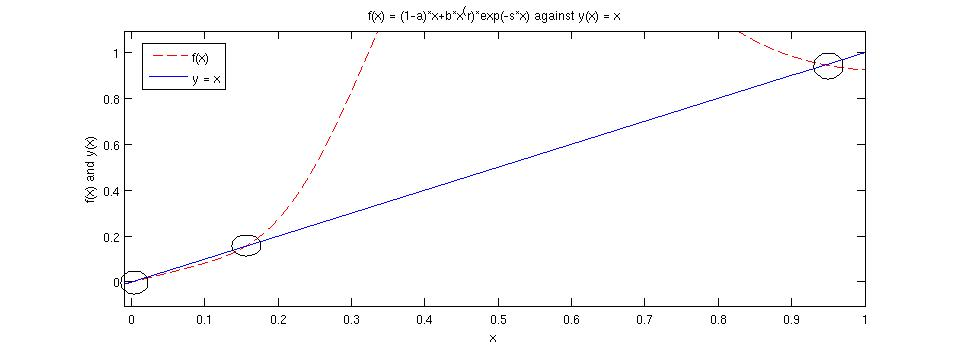
\includegraphics[width=\textwidth]{P1_Q2}
    \end{center}
    \caption{Here we can see that there are at least three fixed points of period one as there are three intersections. Note: the graph has cut off the top of the function for the sake of seeing the intersection points. The behavior of the function is simply concave and reprsents something close to a parabola in this window. For a further picture, see the attached graph at the end of this section.}
    \label{figure:2.1}
\end{figure}

Using Matlab's ``data cursor'' we can identify these points as $x\text{*}_{1} = 0$, $x\text{*}_{2} = 0.16$ and $x\text{*}_{3} = 0.94$. The next step in our analysis is to find the stability at these points.

Determining Stability: Stability at these fixed points is determined by calculating the absolute value of the derivative at the fixed points. If this value is less than 1, then the fixed point is stable; if it is greater than 1, then the fixed point is unstable. In other words,

\begin{align*}
abs(f'(x\text{*})) &< 1 \rightarrow \text{fixed point is stable} \\
abs(f'(x\text{*})) &> 1 \rightarrow \text{fixed point is unstable}
\end{align*}

For this system in general, we find that the derivative is:

\begin{align*}
	\frac{df}{dx\text{*}} &= (1-a) + bx\text{*}^{r}e^{-sx\text{*}}\frac{r-sx\text{*}}{x\text{*}} \text{ and that} \\
	\frac{df}{dx\text{*}} &< 1 \text{ when } a > bx\text{*}^{r-1}e^{-sx\text{*}}(r-sx\text{*})
\end{align*}

In our case, we have used Matlab's symbolic toolbox to calculate the derivatives, seen as `derivf = diff(f)' in the code above. We can then calculate the absolute value of the derivatives at those points yielding the following results:

\pagebreak

\begin{table}[h]
\centering
\begin{tabular}{rrr}
Fixed Point & Abs(f'(x*)) & Stability \\
0           & 0.8000      & stable    \\
0.16        & 2.0418      & unstable  \\
0.94        & 0.6759      & stable   
\end{tabular}
\end{table}

Thus, we have shown that there are two stable fixed points and one unstable fixed point within this system when $a = 0.2$.

\textbf{Question 3:} Assuming that $b=1.1*10^{6}$, $r=8$ and $s=16$ show that there are one stable and two unstable fixed points of period one when $a=0.3$.

\textbf{Answer:} We use the same techniques as the last problem in order to show this to be true.

Here is the graph that is generated by plotting $y=x$ against our $g(x) = (1-a)x+(1.1*10^{6})x^{8}e^{-16x}$ where $a = 0.3$: 

\begin{figure}[H]
    \begin{center}
    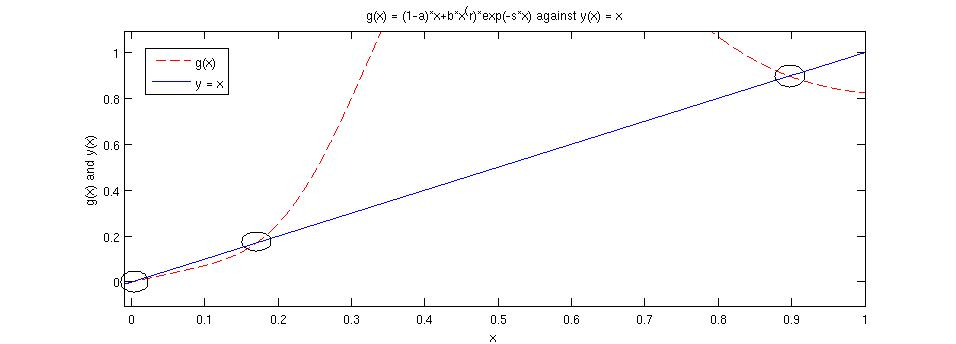
\includegraphics[width=\linewidth]{P1_Q3}
    \end{center}
    \caption{Here, again, we can see that there are at least three fixed points of period one as there are three intersections.}
    \label{figure:2.1}
\end{figure}

Upon analysis with Matlab's `data cursor', it was found that the fixed points seem to differ slightly with values of $x\text{*}_{1} = 0$, $x\text{*}_{2} = 0.17$ and $x\text{*}_{3} = 0.89$. Taking the derivatives at these points yields the expected results of two unstable fixed points and one stable fixed point: 

\begin{table}[h]
\centering
\begin{tabular}{rrr}
Fixed Point & Abs(g'(x*)) & Stability \\
0           & 0.7000      & stable    \\
0.17        & 2.2700      & unstable  \\
0.89        & 1.2859      & unstable   
\end{tabular}
\end{table}

\section*{Complete Diagram of Function from $x = -0.1 \text{ to } 1$}
\begin{figure}[H]
    \begin{center}
    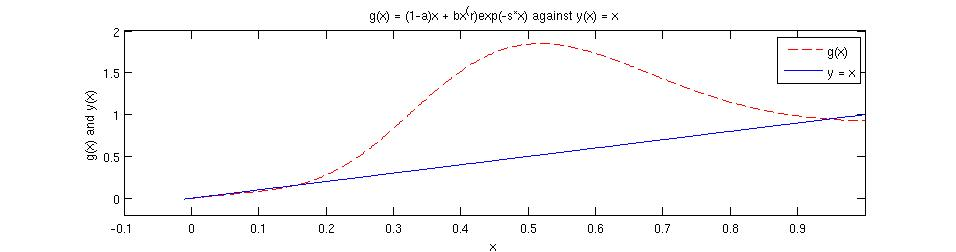
\includegraphics[width=\linewidth]{P1_CompleteGraph}
    \end{center}
    \caption{Here we see the complete graph of the function, particularly the parabolic aspect which was cut off in the previous pictures.}
    \label{figure:2.1}
\end{figure}

\end{document}

